\documentclass{amsart}
\usepackage[style=alphabetic,backend=biber,sorting=nty]{biblatex}
\addbibresource{biblio.bib}
\usepackage[T1]{fontenc}
\usepackage[french,english]{babel}
\usepackage[margin=0.6in]{geometry}
\usepackage{macros}
\usepackage{csquotes}
\usepackage{subfiles, caption, listings}
\usepackage[]{amsmath}
\usepackage{amssymb}
\usepackage{dsfont}
\usepackage{stmaryrd}
\usepackage{hyperref}
\usepackage{graphicx}
\usepackage{varwidth}
\usepackage{float}
\usepackage{amsthm}
\usepackage{verbatim}
\usepackage{enumitem}
\usepackage[most]{tcolorbox}
\usepackage[ruled]{algorithm2e}
\usepackage{relsize}
\usepackage{mathtools}
\usepackage{csquotes}
\usepackage{wrapfig}
\usepackage[colorinlistoftodos]{todonotes}
\renewcommand\thesection{\arabic{section}}

\newcommand{\lref}[1]{\mbox{\thref{#1}}}

%THEOREMS
\theoremstyle{definition}
\newtheorem{definition}{Definition}

\theoremstyle{plain}
\newtheorem{theorem}{Theorem}
\newtheorem{lemma}{Lemma}

\setlist[enumerate,1]{label={(\roman*)}}

\date{December 20, 2024}
\title{Waltz right turn with a Humanoid Robot using Inverse Kinematics}
\author{Constantin Vaillant-Tenzer, Charles Monté}

\begin{document}

\maketitle


\section{Introduction}

Our goal was to code a robot able to dance a waltz right turn using inverse kinematics. To do so, we first implemented a movement acquisition pipeline adapted from various research papers to get the position of joints of interest (feet, pelvis, hands, and head) over time. We then used the joint positions to solve inverse kinematics on a humanoid robot, forcing the robot's joints to follow the ideal positions. Finally, we adapted the rhythm of the movement to fit the BPM of a chosen music.

\section{Previous works}
Waltz dancing is not a common research topic among dancing robots. However, to help robots learn how to dance, there are some already known methods like \textbf{learning from observation}\cite{traditional_jap_dance} where the robot chooses from a series of leg tasks the good ones to imitate a dancing human; or \textbf{real-time gesture responsive frameworks}\cite{spectacle_imitation} where the robot generates unpredictable artistic responses to a dancer's movements.

Concerning waltz dancing, a \textbf{dance partner robot}\cite{ballroom_dance} has been developed to realize human-robot coordination by estimating the next intended movement of a human through physical interaction.

\section{Our method}
\subsection{Overview of the method}
We did not have sufficient time to implement everything ourselves from kinematics acquisition to inverse kinematics solving so we decided to center ourselves around acquiring a good base for the movement kinematics. 
\\

Thus, we mainly relied on already implemented blocks to fit inside our pipeline while trying to get the best approximation of a waltz right turn possible.
\\

The global pipeline we followed for our implementation is represented in Figure 1.

\begin{figure}
  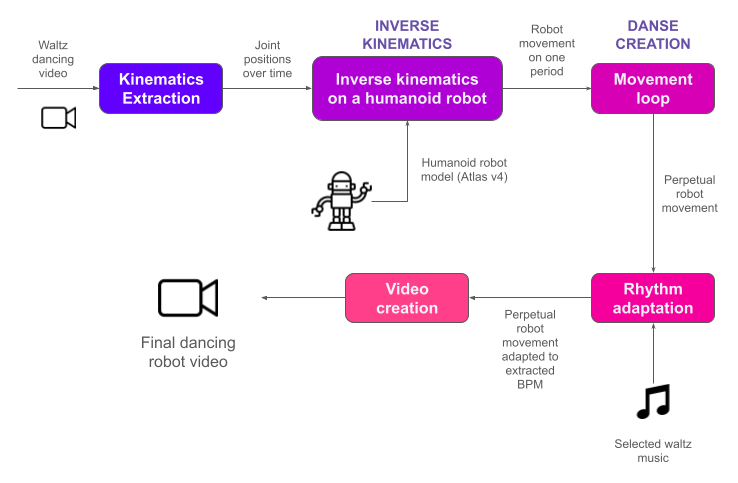
\includegraphics[width = 0.75 \columnwidth]{img/final_solution_pipeline.png}
  \caption{Our approach's full pipeline}
\end{figure}

\subsection{Kinematics Extraction}
Our first idea of Kinematics Extraction was to both extract joint positions and joint angles, to ensure a perfect movement for the robot throughout the waltz movement. This idea did not work in the end, which made us go back to only joint position extraction while putting no constraints on the robot's joint angles, to make the inverse kinematics process find the optimal joint angles itself. In this subsection, we are going to chronologically follow our thought process and implementations of kinematics extraction.
\\

We first decided to focus on two methods, one was proposed by Stéphane Caron at the start of the project : Estimating 3D Motion and Forces of Person-Object Interactions From Monocular Video\cite{Li_2019}, and the second was discovered during research about state-of-the-art kinematics extraction algorithms: NIKI, Neural Inverse Kinematics with Invertible Neural Networks for 3D Human Pose and Shape Estimation\cite{li2023niki}.
\\

We did not focus long on the first method as its implementation was made using outdated projects (HMR for instance) which made the global implementation too tiresome. NIKI on the other hand was perfect for us, as it extracted both the joint positions and the joint angles at the same time. While the joint positions were easy to understand and use (with some tinkering to find each Joint Id - see NIKI results exploitation notebook in the GitHub), the joint angles did not follow a shape we understood. We were provided with fewer angles than the number of joints and no idea of which joint they were related to. We did not manage to understand how to extract each joint's angle over time, even after carefully reading the related paper and source code. 
\\

\begin{figure}
  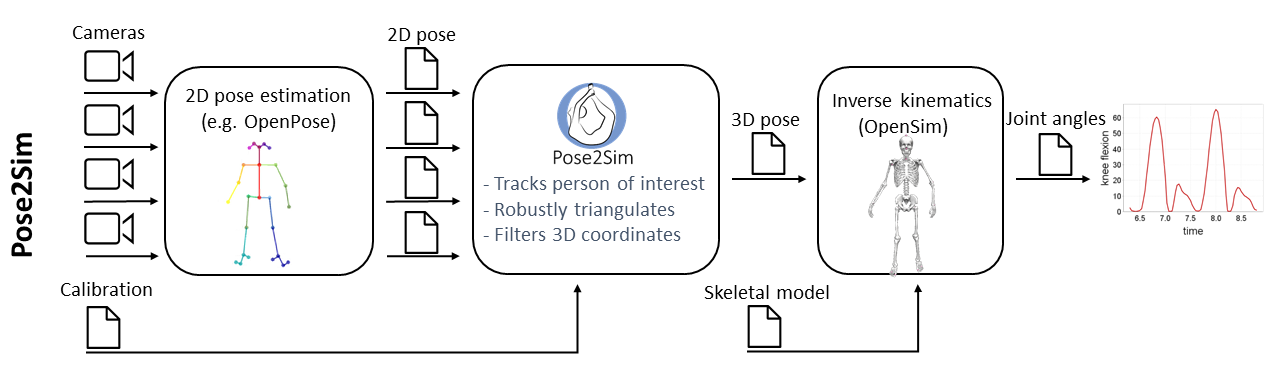
\includegraphics[width = 0.99 \columnwidth]{img/pose2sim_pipeline.png}
  \caption{The Pose2Sim pipeline : This solution extracts 2D keypoints coordinates (using RTM Pose\cite{RTMPose}) to produce an OpenSim result (full-body 3D joint angles), which we use in our pipeline by extracting the information that is interesting from us, ie. the RTMPose output and the full-body 3D joint angles. }
\end{figure}

Thus, we decided to find a new pipeline that could extract both, in an intelligible manner: Pose2Sim\cite{Pose2Sim}. Pose2Sim has been the main pipeline we have used for the extraction of joint positions and angles, mainly because the outputs were directly linking each joint name to an angle and a position. Pose2Sim's global pipeline can be found in Figure 2. This solution is not that different from the two proposed above, they follow a similar chain of thought which consists of a 2D pose estimation algorithm (RTM Pose\cite{RTMPose} for Pose2Sim), followed by a block that projects those coordinates to the 3D space, before doing inverse kinematics to find the optimal joint angles to adapt the joint positions to a humanoid model. 
\\

Even if only using the first part of all those implementations to extract the 3D joint positions before using our own Inverse Kinematics to get the optimal joint angles now seems obvious, we lost a lot of time trying to use both the joint positions and angles to try and get a perfect movement. We first implemented a global pipeline using the Pose2Sim results, which we presented during the poster session. It did not work due to bad adaptations of the joints to the angles and the positions, which blocked the robot in place, only allowing its feet to move. 
\\

After reflecting on our implementation, we managed to make the robot move but noticed that both the Pose2Sim and NIKI extracted joint positions were not parallel to the $(x, y)$ plane. Thus, we decided to find optimal transformation matrices (composition of rotations, translations, and scaling for the $x$, $y$, and $z$-axis) but did not manage to find one, manually or with optimization algorithms, to make Pose2Sim results exploitable. The reasons we identified for it were two-fold.

\begin{enumerate}
    \item The transformation applied to the movement was too difficult for us to estimate manually and we did not manage to find optimal cost algorithms to have a good transformation matrix output.
    \item The Pose2Sim pipeline adapts the joint positions to the 3D space with the use of the extrinsic and intrinsic camera parameters while assuming that the camera is static. However, in the video we used, the camera moves during the acquisition which throws off the Pose2Sim estimation causing a huge change in $x,y,z$ coordinated in the middle of the movement, as seen in Figure 3.
\end{enumerate}
\\

What finally worked was to only use the joint positions extracted thanks to the NIKI algorithm, pre-processing them using smoothing functions for each coordinate and making them parallel to the $(x, y)$ plane, and then solving inverse kinematics using those joint positions to find the optimal angles automatically. 

\subsection{Inverse Kinematics}

TODO

To solve the inverse kinematics, we applied Pink (\cite{pink2024}) which solves differential inverse kinematics by weighted tasks. 
\\ 

The method uses \textbf{residual functions} of the robot configuration $q$ that should be driven to zero to make the robot do a certain task. In our case, we for instance try to put the robot's feet at a certain position $p_{\text{feet}}^*$ so an example of a residual would be $e(q) = p_{\text{feet}}^* - p_{\text{feet}}(q)$. 
\\

To solve the equation system produced, the method computes a velocity $v$ that satisfies the equation $J_e(q)v = \dot{e}(q) = -\alpha e(q)$ - $J_e(q)$ being the Jacobian of task $e$ - for each residual. 
It is of course not possible so the method finds the optimal solution to the following minimization problem, which finds the movement which tries to solve all of the tasks at the same time.
$$
\begin{aligned}
\min_v \ \ &\sum_{\text{tasks} \ e} ||J_e(q)v + \alpha e(q)||^2 \\
\text{subject to} \ \ \ &v_{min}(q) \leq v \leq v_{max}(q)
\end{aligned}
$$

\begin{figure}
  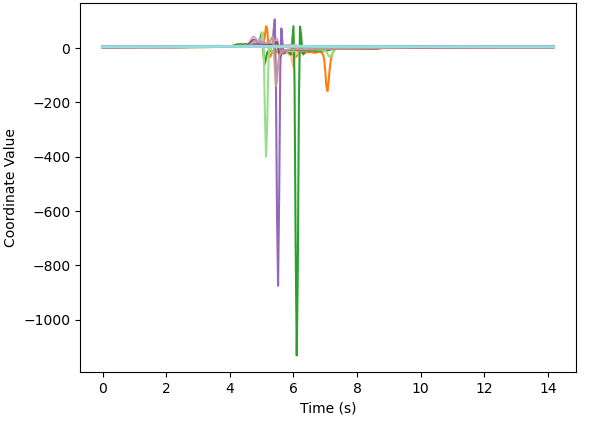
\includegraphics[width = 0.5 \columnwidth]{img/x_coord_pose2sim.png}
  \caption{x-coordinate of each joints over time with Pose2Sim extraction}
\end{figure}

\printbibliography

\end{document}